\section{Why: what the $K$-step reward is and does}
\label{sec:mechanism}

Everything here is measured on the training oracle at branching time (the held-out judge never
scored a training candidate), at a fixed policy where possible.

\paragraph{Look-ahead rescales the training signal; it does not sharpen it.} With \Kf{} every
dispersion statistic of the group of eight rises. At the base policy (training iteration~1,
where both $K$ arms branch from the same $\pi_0$) the \Kf{}/\Kz{} ratio of the mean best--worst
margin is $1.55$ for PTO and $1.44$ for GRPO --- but the ratio of the within-group SD is $1.53$
and $1.40$, so the ratio of ratios is $1.01$ [$1.00$, $1.03$] and $1.03$ [$1.02$, $1.04$]
(Figure~\ref{fig:dispersion}, Appendix~\ref{app:tails}). Look-ahead widens the spread and barely
moves the best candidate relative to the pack: the winner's standardized lead is higher under
\Kf{} by only $0.07$ SD (PTO, base; $-0.00$ pooled) and $0.16$ SD (GRPO, base; $+0.10$ pooled)
against a $1.4$--$1.5\times$ scale effect (Appendix~\ref{app:tails}). GRPO's group normalization divides that scale straight back out. PTO's
absolute $\tau{=}0.1$ does not: pair yield at the base policy is $0.935$ under \Kf{} against
$0.824$ under \Kz{}, and multiplying the \Kz{} margins by the SD ratio $1.53$ lifts \Kz{} to
$0.872$ --- $0.437$ of the gap is the rescaling. The selection also has a direction: PTO \Kf{}
is the only arm whose update favours longer completions at every training iteration (its length
push $w_{\text{len}}$ --- the completion-length contrast the update rewards, in characters:
chosen minus rejected for DPO, advantage-weighted for GRPO --- is positive throughout, $+49.5$ to
$+7.0$ chars, SE $7$--$14$, at least $2.3$ SE from zero at iterations 1--9 and $0.96$ SE at
iteration~10; PTO \Kz{}'s never exceeds $1.7$ SE from zero), the training-side counterpart of the session-shape reversal in
\S\ref{sec:behaviour}.

\paragraph{At a matched policy the $K$-step reward is no more faithful.} In our runs the reward
at the shortest cut ($\text{MCL}{=}12$) already ranks conversations like the full-conversation \QQ{}
well above chance for every arm (pairwise sign agreement $0.86$--$0.89$, same grader), and at
the base policy the \Kz{}$-$\Kf{} agreement delta is $+0.004$ [$-0.067$, $0.074$] for PTO and
$+0.015$ [$-0.023$, $0.057$] for GRPO; the \Kf{} lead when all iterations are pooled (PTO
$-0.027$ [$-0.047$, $-0.006$]) is a trajectory effect (Figure~\ref{fig:faithfulness}).

\begin{figure*}[t]
  \centering
  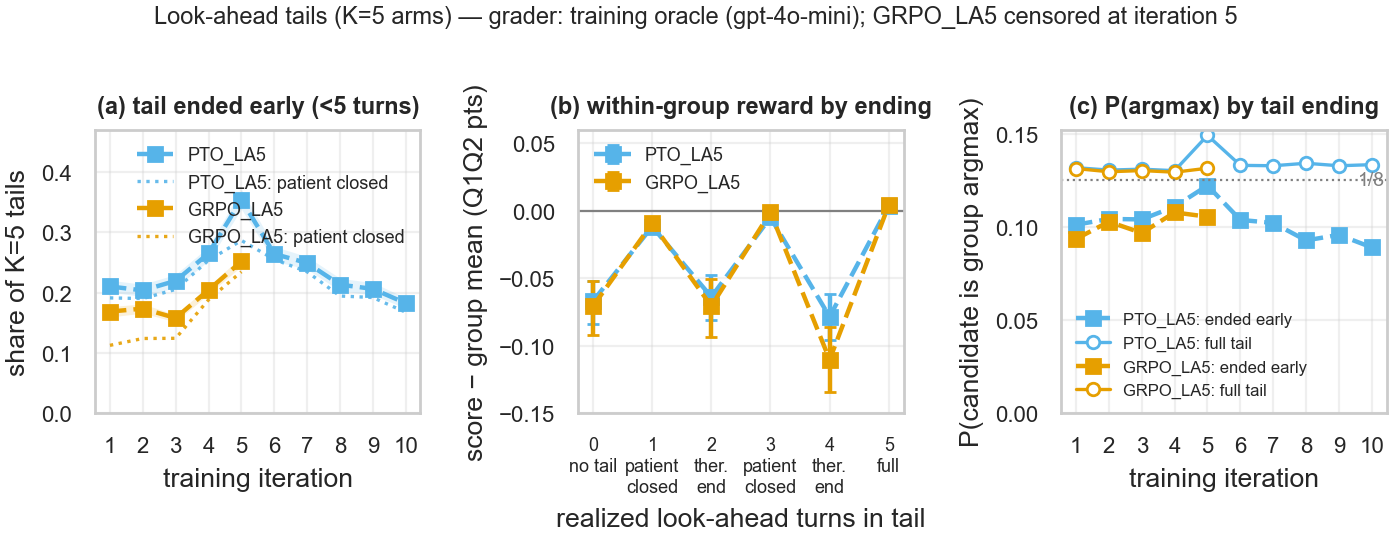
\includegraphics[width=0.96\textwidth]{figures/tail_audit_fig.png}
  \caption{The look-ahead tails (both \Kf{} arms, labelled LA5 in the legend; training oracle).
    (a) Share of tails cut short
    of five turns, and the share due to the patient closing. (b) Within-group score deviation by
    realized tail length (odd $=$ patient closed; even $=$ therapist-final; $0$ $=$ no tail).
    (c) P(group argmax) for ended-early vs.\ full tails; $1/8$ is chance. GRPO \Kf{} ends at
    iteration~5.}
  \label{fig:tails}
\end{figure*}

\paragraph{What the tail contains.} About one \Kf{} tail in five is shorter than five turns ---
$22.8\%$ of $59{,}868$ PTO candidates and $19.2\%$ of $55{,}552$ GRPO candidates --- almost
always because the simulated patient closes the session ($21.1\%$ / $16.1\%$ of candidates);
failure tails (no reply, stalled therapist, therapist-final) are $2$--$3\%$.
Within the group the update sees, ended-early siblings score lower than full-tail siblings by
$0.034$ points for PTO ($\dz{=}{-}0.24$, $3{,}809$ groups) and $0.051$ for GRPO
($\dz{=}{-}0.25$), Holm-significant in every iteration, and are $21$--$23\%$ less likely to be
the argmax (RR $0.77$ [$0.74$, $0.80$] / $0.79$); in PTO that pressure grows over training (RR
$0.77 \to 0.67$). The penalty falls on the rare failure tails ($-0.06$ to $-0.11$), not on
patient closes ($0.00$ to $-0.01$; Figure~\ref{fig:tails}b; Appendix~\ref{app:tails}).

\paragraph{$K$ acts through the data, not the loss.} Under \Kf{} the two optimizers' pooled
update directions (each arm's iterations pooled; GRPO \Kf{} 1--5, the others 1--10) align far
more (attenuation-corrected cosine $0.74$ vs.\ $0.32$ under \Kz{}). Swapping the weighting rule
(best-vs-worst $\leftrightarrow$ group-relative) on fixed data leaves the direction almost
unchanged (raw cosine $0.91$--$0.99$); swapping the data under a fixed rule reproduces the gap
(corrected $0.73$ under \Kf{}, $0.32$--$0.40$ under \Kz{}). The lever
changes what is scored, and that is what the two optimizers inherit. Separately, the training oracle under-reports the harm channel: gain
retention on MI-inconsistency ($\Delta$ held-out $/$ $\Delta$ oracle over own base) exceeds $1$
in every defined cell from iteration~3 on for all four arms ($1.06$--$4.63$; the CI excludes $1$
in all but four cells; endpoints PTO \Kz{} $1.66$, PTO \Kf{} $2.44$, GRPO \Kf{} at iteration~5
$2.44$, GRPO \Kz{} at iteration~10 $1.06$ [$0.94$, $1.21$]), so whatever
look-ahead does to this channel reaches the optimizer attenuated.
